\chapter{Alternatieve Logische Systemen}\label{ch:systemen}
In de hoofdsectie van Logica en Wiskunde hebben we kennis gemaakt met klassieke (propositie/predicaten)-logica, maar dit is lang niet het enige logische systeem. In dit hoofdstuk introduceren we het belangrijkse alternatief, intu\"itionistische logica, en zullen we een aantal andere systemen in vogelvlucht behandelen.

Gezien vanaf klassieke logica kunnen alternatieve systemen in twee belangrijke manieren verschillen:
\begin{enumerate}
  \item het systeem voegt iets toe aan de taal van de logica, of
  \item het systeem vervangt de notie van \enquote{waarheid} door een ander onderwerp.
\end{enumerate}
De eerste variant uit zich doorgaans in extra notatie en axioma's om deze te verankeren, de tweede door het vervangen of verwerpen van axioma's: stelling die in de klassieke logica zonder bewijs worden aangenomen om als uitgangspunt voor andere theori\"en te dienen werken niet in deze logica's. Merk op dat de meeste logica's in een van deze twee punten afwijken ten opzichte van klassieke logica, maar dat het ook mogelijk is dat beiden simultaan van toepassing zijn. Daarnaast is het mogelijk om een of meerdere toevoegingen aan de taal te combineren met altijd \'e\'en set axioma's. Wij zijn bijvoorbeeld begonnen met klassieke propositie-logica, die we vervolgens hebben uitgebreid met predicaten. Diezelfde predicaten kunnen we ook toevoegen aan bijvoorbeeld intu\"itionistische logica. De interpretatie van de nieuwe notatie zal zich dan aanpassen naar de betekenis van proposities in de doel-logica. In Sectie~\ref{sec:modal} zullen we modale logica als toevoeging bovenop een propositielogica zien, dit kan op basis van zowel klassieke als intu\"itionistische logica, en werkt onafhankelijk van de aanwezigheid (of niet) van predicaten.

\section{Intu\"itionistische Logica}\label{sec:il}
Waar klassieke logica proposities gebruikt om de waarheid van logische zinnen na te gaan, laten we het concept van waarheid in intu\"itionistische logica (IL) los en kijken we in plaats daarvan naar bewijs. Dit is een hardere eis, wat betekent dat de intu\"itionistische logica minder stellingen bevat die echter wel sterker onderbouwd zijn. Waar we in klassieke logica een stelling kunnen bewijzen door aan te tonen dat het tegendeel onwaar is, kan dat in klassieke logica niet\sidenote{Het axioma dat $P \equiv \neg \neg P$ werkt niet in IL, enkel de gevolgtrekking $\neg \neg P \vdash P$. Ik mag niet uit een dubbele ontkenning een bewijs halen, maar kan wel een dubbele ontkenning introducren.}. Dit volgt direct uit de andere interpretatie van proposities: waarheid is binair, dus als iets niet onwaar is, moet het waar zijn. Bewijs moet daarentegen getoond kunnen worden, dus de stelling dat ik niet kan bewijzen dat er geen bewijs voor mijn aanname is, is niet zo overtuigend.

De andere interpretatie heeft een aantal directe gevolgen, bijvoorbeeld dat een deel van onze bewijssystemen wegvalt of verandert: waarheidstabellen zijn niet op IL van toepassing, en de boom-methode wordt iets minder ergonomisch. De sequenten-calculus en natuurlijke deductie werken zoals we gewend zijn, behalve dat een aantal regels veranderen. Het systeem \lk{} wordt \textsf{LJ}, met als voornaamste verchil dat er maximaal \'e\'en stelling rechts van de peil mag staan, en dat we de negatie-regels zullen moeten aanpassen. Meestal wordt dit opgelost door negatie niet als aparte connectief te zien, maar als een shorthand voor \enquote{impliceert onwaar}: $\neg P$ wordt behandeld als $P \to \bot$. Voor natuurlijke deductie verdwijnen een aantal regels (waarmee klassieke logica gezien kan worden als een uitbreiding op de intu\"itionistische).

Om vanuit IL naar klassieke logica te komen volstaat het om de regel van dubbele negatie eliminatie (DNE) te (her)introduceren, maar dat is hiet de enige mogelijkheid. Een andere belangrijke regel uit de klassieke logica die niet geldig is in IL, is de wet van het uitgesloten midden (LEM): in klassieke logica kan ik ten alle tijde aannemen dat $P \lor \neg P$, in IL mag dit niet. Wederom: in termen van waarheid is een stelling waar of niet waar, maar het is niet zo dat deze bewezen waar of onwaar is. Het blijkt dat de het voldoende is om DNE aan te nemen om LEM te bewijzen, of vice versa. Een derde stelling met deze eigenschap is de wet van Peirce $((P \to Q) \to P) \to P$. Alledrie deze stellingen zijn ongeldig in IL, maar het introduceren van \'e\'en is voldoende om de andere twee af te leiden.

\section{Constructieve Wiskunde}
Intu\"itionistische logica heeft een nauwe band met de constructieve wiskunde. Een hoofdonderwerp in de wiskunde is het bewijzen van stellingen over getallen, ruimtes, vormen, etc. Constructieve bewijzen moeten de eigenschap hebben dat ze op z'n minst \'e\'en voorbeeld (ook wel \emph{getuige}) van de bewezen stelling laten zien.

Een gebruikelijke bewijstechniek, die binnen de constructieve wiskunde wordt verworpen, is het bewijs met contradictie. De vorm waarin bewezen wordt dat een stelling onwaar is, werkt (er is geen voorbeeld, dus dit kunnen we niet verwachten), maar de vorm waarin bewezen wordt dat een stelling waar is, omdat deze niet onwaar is, is niet geldig, omdat hier de getuige uit ontbreekt. Ook de vorm waarin we LEM gebruiken om te stellen dat een (deel)-stelling waar of onwaar moet zijn, is ongeldig.

\begin{example}\label{ex:nonconstr}
Neem bijvoorbeeld de stelling "Er bestaan irrationele (re\"ele) getallen $a$ en $b$ zodat $a^b$ een rationeel getal is. In de klassieke wiskunde is dit te bewijzen door het geval $\sqrt{2}^{\sqrt{2}}$ te nemen. We weten dat $\sqrt{2}$ irrationeel is, dus dit kunnen we nemen als $a$ en $b$. Nu kan het zo zijn dat $\sqrt{2}^{\sqrt{2}}$ rationeel is, of niet (LEM). In het eerste geval zijn we klaar, in het tweede geval kiezen we $a = \sqrt{2}^{\sqrt{2}}$ en $b = \sqrt{2}$. Van beide weten we dat deze irrationeel zijn (als $a$ rationeel was, dan waren we niet in dit stuk van het bewijs), maar als we $a^b$ versimpelen met de exponent-regel krijgen we 
  $$\left(\sqrt{2}^{\sqrt{2}}\right)^{\sqrt{2}} = \sqrt{2}^{(\sqrt{2}\cdot\sqrt{2})} = \sqrt{2}^2 = 2 \in \mathbb{Q}$$\\
\hfill\qed
\end{example}

Het gegeven bewijs werkt binnen de klassieke wiskunde, maar niet binnen de constructieve wiskunde; technisch gezien door de toepassing van LEM, praktisch gezien omdat het bewijs geen getuige heeft waarvan bewezen is dat dat het rationele getal $a^b$ is\sidenote{Om van dit bewijs een geldig constructief bewijs te maken zou moeten worden aangetoond welke optie de juiste is, waarmee een concreet voorbeeld wordt gegeven. In dit geval is een concreet voorbeeld het meest voordehandliggend, maar in veel gevallen is een bewijs een algoritme of recept om voorbeelden te genereren.}.

\section{Type-theorie}
In Hoofdstuk~\ref{ch:verzamelingen} hebben we kennis gemaakt met verzamelingen. Types vormen, wiskundig gezien, een vergelijkbaar concept, met een aantal verschillen om bijvoorbeeld paradoxen\sidenote{Bijvoorbeeld Russel's Paradox: Laat $R$ de set zijn van alle sets die niet zichzelf bevatten. Zit $R$ wel of niet in zichzelf?} te voorkomen. In type-theorie zijn waardes en types onlosmakelijk verbonden: waar een element in meerdere verzamelingen kan zitten, heeft het een enkel type (notatie $x : A$, $x$ heeft het type $A$ / is een bewoner van het type $A$). De waardes $2 : \mathbb{N}$ en $2 : \mathbb{Z}$ zijn daarmee bijvoorbeeld verschillende entiteiten geworden, die wel gelijkwaardig zijn maar niet hetzelfde.

In IL worden proposities gezien als bewijzen, wat betekent dat we hier niet langer een valuatie $0$ of $1$ aan kunnen geven zoals in klassieke logica. In plaats daarvan wordt, via het Curry-Howard isomorfisme, een propositie gezien als een type, dat de getuigen bevat van de stelling waar de propositie naar verwijst. Een stelling zonder bewijs is het lege type en komt overeen met $\bot$ in de logica, $\top$ komt overeen met het type met een enkel bewijs (alle bewijzen zijn hetzelfde, \enquote{waarheid is waar}). $\bot$ en $\top$ hebben niet de waardes $0$ en $1$, maar wel respectievelijk $0$ en $1$ getuigen / termen. 

Logische operatoren komen overeen met manieren om de bewijzen te combineren, en de logische regels met programmeerconcepten.  De conjunctie komt overeen met heb producttype, dat we in deze context doorgaans als $A \times B$ schrijven in plaats van $A \land B$. In Python-termen is dit het tuple \textsf{(a, b)}. Op dezelfde manier wordt disjunctie het somtype $A + B$, een type dat zowel $A$ als $B$ mag zijn\sidenote{Dit type vertaalt zich niet goed naar Python, omdat Python niet statisch getypeerd is, en variabelen dus altijd van type kunnen wisselen. In statisch getypeerde talen kan dit niet, en heeft een variabele \'e\'en type. Met het somtype kunnen we aangeven dat een variabele in zo'n geval bijvoorbeeld \textsf{bool} of \textsf{str} is, en op basis van het type bepaalde code uitvoeren. Op dezelfde manier is het verschil tussen tuples en lijsten in dergelijke talen duidelijker: een lijst bevat een (in de regel niet beperkt) aantal items van \'e\'en en hetzelfde type, een tuple bevat twee items die elk hun eigen type hebben (dat mag tweemaal hetzelfde type zijn, maar hoeft niet).}. Implicatie wordt als functietype nog steeds als $A \to B$ geschreven, en negatie is zoals eerder gezegd vervangen door implicatie van $\bot$.

\begin{figure}[ht]
\begin{theorem}\label{th:nd-il} Natuurlijke Deductie voor IL
\paragraph{Axioma's}\mbox{}\\[3mm]
\inference{Id}{}{x : A \vdash x : A}

\paragraph{Structurele Regels}\mbox{}\\[3mm]
\inference{W}{\Gamma \vdash u : B}{\Gamma, x : A \vdash u : B}
\hspace{5mm}
\inference{C}{\Gamma, y : A, z : A, \vdash u : B}{\Gamma, x : A \vdash u[x/y, x/z] : B}
\hspace{5mm}
\inference{E}{\Gamma, \Delta \vdash t : A}{\Delta, \Gamma \vdash t : A}

%\paragraph{Cut Rule}\mbox{}\\[3mm]
%\fork{}{\Gamma \vdash A}{\Sigma, A, \Pi \vdash \Delta}{\Sigma, \Gamma, \Pi \vdash \Delta}

\paragraph{Logische regels}\mbox{}\\[3mm]
\inference{\to I}{\Gamma, x : A \vdash u : B}{\Gamma \vdash \lambda x. u : A \to B}
\hspace{5mm}
\fork{\to E}{\Gamma \vdash s : A \to B}{\Delta \vdash t : A}{\Gamma, \Delta \vdash s(t) : B}

\vspace{4mm}

\fork{\times I}{\Gamma \vdash t : A}{\Delta \vdash u : B}{\Gamma, \Delta \vdash (t, u) : A \times B}
\hspace{5mm}
\fork{\times E}{\Gamma \vdash s : A \times B}{\Delta, x : A, y : B \vdash v : C}{\Gamma, \Delta \vdash \text{case } s \text{ of } (x, y) \to v : C}

\vspace{4mm}
\inference{+I_1}{\Gamma \vdash t : A}{\Gamma \vdash \text{inl}(t) : A+B}
\hspace{5mm}
\inference{+I_2}{\Gamma \vdash v : B}{\Gamma \vdash \text{inr}(v) : A+B}

\vspace{4mm}

\trifork{+E}{\Gamma \vdash s : A + B}{\Delta, x : A \vdash v : C}{\Delta, y : B \vdash w : C}{\Gamma, \Delta \vdash \text{case } s \text{ of inl}(x) \to v; \text{ inr}(y) \to w : C}

\end{theorem}
\end{figure}

In Stelling~\ref{th:nd-il} zijn de natuurlijke deductie regels voor intu\"itionistische logica weergegeven, met de bijbehorende types. De regels voor IL komen overeen met een subset van de regels die voor klassieke logica hebben gezien. 

We kunnen nu het bewijs uit Voorbeeld~\ref{ex:nd:export} nog eens bekijken, ditmaal met de types ingevuld. Hoewel we dit bewijs hebben gegeven in de klassieke logica, valt dit geheel in het fragment dat met IL overeen komt en kunnen we dit dus ook in IL opvoeren. We kunnen nu termen aan de axioma's toevoegen, en van onder naar boven de term van de laatste bewijsstap achterhalen.

\begin{example}\label{ex:typed}
\begin{prooftree}
  \ndax{$f : (P \times Q) \to R \vdash f : (P \land Q) \to R$}
    \ndax{$x : P \vdash x : P$}
    \ndax{$y : Q \vdash y : Q$}
  \ndprodi{$x : P, y : Q \vdash (x, y) : P \times Q$}
\ndimple{$f : (P \times Q) \to R, x : P, y : Q \vdash f (x, y) : R$}
\ndimpli{$f : (P \times Q) \to R, x : P \vdash \lambda y. f(x, y) : Q \to R$}
\ndimpli{$f : (P \times Q) \to R \vdash \lambda x. \lambda y. f(x, y) : P \to (Q \to R)$}
\ndimpli{$\vdash \lambda f\!. \lambda x. \lambda y. f(x, y) : ((P \times Q) \to R) \to (P \to (Q \to R))$}
\end{prooftree}
\end{example}

Met de termen erbij ontstaat een lambda-functie, die in de functionele wereld bekend staat als \texttt{curry} en die we in Python kunnen opschrijven als \verb|curry = lambda f: lambda x: lambda y: f(x, y)|. Deze functie pakt steeds een argument per keer, eerst een functie en dan twee argumenten, en past de functie op beide argumenten toe. \verb|curry(min)(2)(3)| rekent $min(2,3) = 2$ voor ons uit. Hoewel deze functie in Python syntax niet bijzonder zinvol is, laat deze zien dat het niet uitmaakt voor een functie of we de argumenten een voor een geven (standaard in veel functionele talen) of in een keer als een tuple (zoals bijvoorbeeld Python dat doet).  Merk op dat we in dit voorbeeld een extra implicatie-introductie hebben gedaan om de functie \texttt{f} als parameter te krijgen.

\subsection{Oefeningen}

\begin{exercise}\mbox{}\\
  Vertaal de bewijzen uit Sectie~\ref{ex:ndc} naar IL, pas een extra implicatie-introductie toe, en voorzie elk bewijs van termen. Probeer per functie onder woorden te brengen wat deze doet.

\begin{enumerate}[label=\textit{\alph*.}]
\item $\vdash ((p + q) \to \bot) \to ( p \to \bot)\times( q \to \bot)$ \\
\item $\vdash ( p \to \bot)\times( q \to \bot) \to ((p + q) \to \bot)$ \\
\item $\vdash ( p \to \bot)  +( q \to \bot) \to ((p\times q) \to \bot)$ \\
\item $\vdash (p + q)\times r \to (p\times r) + (q\times r)$ \\
\item $\vdash (p\times r) + (q\times r) \to (p + q)\times r$  \\
\item $\vdash (p\times q) + r \to (p + r)\times(q + r)$ \\
\item $\vdash (p + r)\times(q + r) \to (p\times q) + r$  \\
\end{enumerate}\vspace{3mm}

\textbf{Hint:} Door de manier van formuleren met functies voor negaties, zul je uiteindelijk termen tegenkomen als $f(p)$ met $f : P \to \bot$ en $p : P$. Dit betekent dat $f(p) : \bot$, wat overeenkomt met een functie-call zonder return --- denk aan een oneindige loop.

\end{exercise}

\begin{exercise}\mbox{}\\
Probeer dit ook voor Voorbeeld~\ref{ex:nd:demorgan}, tot welke stap is het bewijs geldig? Stel vast dat het niet lukt de stelling te bewijzen (de stelling is ongeldig in IL). Onderbouw waarom dit het geval is, door te benoemen welke stappen ontbreken en wat de stelling in de semantiek van IL (proposities als bewijzen) zou betekenen.
\end{exercise}

\section{Substructurele Logica}
Niet elke logica onderschrijft dezelfde structurele regels: weakening, contraction en exchange. Voor werken met binaire waarheden werken deze regels goed, maar zodra aantal of volgorde een rol van betekenis krijgt maken deze regels onwenselijke zinnen geldig. Een substructurele logica is een logica die \'e\'en of meerdere structurele regels verbiedt of beperkt.

\subsection{Lineaire Logica}
Met klassieke en intu\"itionistische logica hebben we gezien dat we logica kunnen inzetten voor verschillende toepassingen (proposities als binaire waarheid of bewijs) met grotendeels overlappende systemen. In lineaire logica beschouwen we proposities als \emph{resources}, die, nadat we ze hebben gebruikt, kunnen verdwijnen. Beschouw, binnen de context van klassieke logica, de zin $T \to P$, met de interpretaties $T$ voor \enquote{ik heb 10 euro} en $P$ voor \enquote{ik heb een pizza}. Als ik nu daadwerkelijk 10 euro heb, ($T$ is waar) mogen we (in non-lineaire klassieke of intu\"itionistische logica) concluderen dat $P$ dat ook is, en dat $T \land P$ daarmee ook het geval is. Dit zou kloppen als geld (en pizza's) geen beperkte resource zijn, maar in de echte wereld zal ik mijn 10 euro moeten inleveren om de pizza te bemachtigen.

Om hier in een logisch systeem mee om te kunnen gaan, moeten we ons eerst de vraag stellen hoe het mogelijk is dat onze 10 euro onuitputtelijk lijkt te zijn. Als we dit bekijken aan de hand van de regels voor natuulijke deductie, dan zien we dat de structurele regels, met name contraction, een voordehandliggende bron van dit probleem zijn. Om tot lineaire logica te komen kunnen we de intu\"itionistische logica als uitgangspunt nemen\sidenote{We formuleren hier eerst een intu\"itionistische lineare logica (ILL); er bestaat ook een klassieke lineaire logica, die iets complexer is dan ILL en het beste begrepen kan worden als uitbreiding op ILL.} en contraction uit onze natuurlijke deductieregels te verbannen. We kunnen dan ook meteen weakening aanpakken, die ons toestaat aannames te laten verdwijnen, wat idealiter ook niet spontaan met mijn 10 euro (of pizza) zou mogen gebeuren. Dit is een goed begin, maar misschien wat weinig flexibel --- uiteindelijk hebben we ook te maken met resources die vrijwel onuitputtelijk zijn\sidenote{Zoals Einstein naar verluid zou hebben gezegd: \enquote{Two things are infinite, the universe and human stupidity, and I am not yet completely sure about the universe.}}, dus maken we een onderscheid tussen lineaire termen (zonder contraction en weakening) en intu\"itionistische termen (met contraction en weakening zoals we gewend zijn).

Dit verandert de betekenis van onze connectieven behoorlijk, waardoor een behoefte aan nieuwe symbolen ontstaat. We vervangen implicatie door $A \multimap B$, en lezen dit als \enquote{neem A om B te verkrijgen}. Conjunctie splitst zich in twee nieuwe operatoren, $A \otimes B$ (multiplicatieve conjunctie) voor \enquote{zowel A als B} en $A \with B$ (additieve conjunctie) voor \enquote{keuze uit A en B}. In de tweede hebben we een resource die we kunnen inzetten om een $A$ of $B$ te krijgen (beide opties zijn mogelijk), maar die we maar eenmaal kunnen gebruiken (waardoor we dus nooit $A$ en $B$ tegelijkertijd hebben). Vergelijk dit verder met disjunctie, $A \oplus B$, die $A$ of $B$ kan bevatten maar waarbij de keuze welke van de twee al tijdens het aanmaken heeft plaatsgevonden\sidenote{In iets concretere termen, $K \otimes T$ is de combinatie van een beker koffie en een beker thee, $K \with T$ is de keuze om een beker koffie of een beker thee te krijgen, en $K \oplus T$ is een afgesloten thermoskan met een verrassing of er koffie of thee in zit.}. Tot slot hebben we de notatie $\oc A$, \enquote{natuurlijk A}, om een resource onbeperkt te maken. Om aan te geven of een aanname lineair of intu\"itionistisch is gebruiken we respectievelijk $\langle A \rangle$ en $\lbrack A \rbrack$.

\begin{figure}[ht]
\begin{theorem}\label{th:nd-ill} Natuurlijke Deductie voor ILL
\paragraph{Axioma's}\mbox{}\\[3mm]

\inference{\langle Id \rangle}{}{\langle A\rangle \vdash A}
\hspace{5mm}
\inference{\lbrack Id \rbrack}{}{\lbrack A \rbrack \vdash A}

\paragraph{Structurele Regels}\mbox{}\\[3mm]

\inference{W}{\Gamma \vdash B}{\Gamma, \lbrack A \rbrack \vdash B}
\hspace{5mm}
\inference{C}{\Gamma, \lbrack A], \lbrack A \rbrack \vdash B}{\Gamma, \lbrack A\rbrack  \vdash B}
\hspace{5mm}
\inference{E}{\Gamma, \Delta \vdash A}{\Delta, \Gamma \vdash A}

\paragraph{Logische Regels}\mbox{}\\[3mm]

\inference{\oc I}{[\Gamma] \vdash A}{[\Gamma] \vdash \oc A}
\hspace{5mm}
\fork{\oc E}{\Gamma \vdash \oc A}{\Delta, \lbrack A\rbrack  \vdash B}{\Gamma, \Delta \vdash B}

\vspace{4mm}

\fork{\otimes I}{\Gamma \vdash A}{\Delta \vdash B}{\Gamma, \Delta \vdash A \otimes B}
\hspace{5mm}
\fork{\otimes E}{\Gamma \vdash A \otimes B}{\Delta, \langle A \rangle, \langle B \rangle \vdash C}{\Gamma, \Delta \vdash C}

\vspace{4mm}

\fork{\with I}{\Gamma \vdash A}{\Gamma \vdash B}{\Gamma \vdash A \with B}
\hspace{5mm}
\inference{\with E_1}{\Gamma \vdash A \with B}{\Gamma \vdash A}
\hspace{5mm}
\inference{\with E_2}{\Gamma \vdash A \with B}{\Gamma \vdash B}

\vspace{4mm}

\inference{\multimap I}{\Gamma, \langle A \rangle \vdash B}{\Gamma \vdash A \multimap B}
\hspace{5mm}
\fork{\multimap E}{\Gamma \vdash A \multimap B}{\Delta \vdash A}{\Gamma, \Delta \vdash B}

\vspace{4mm}
\inference{\oplus I_1}{\Gamma \vdash A}{\Gamma \vdash A\oplus B}
\hspace{5mm}
\inference{\oplus I_2}{\Gamma \vdash B}{\Gamma \vdash A\oplus B}

\vspace{4mm}

\trifork{\oplus E}{\Gamma \vdash A \oplus  B}{\Delta, \langle A \rangle \vdash C}{\Delta, \langle B \rangle \vdash C}{\Gamma, \Delta \vdash C}
\end{theorem}
\end{figure}

\begin{aside}[Klassieke Lineaire Logica]
  De hierboven beschreven logica is slechts een voorbeeld van de verschillende lineaire logica's, specifiek het positieve\sidenote{Een positief fragment van een logica bevat geen regels voor negatie.} fragment van een intu\"itionistische lineaire logica. Voor een klassieke lineaire logica zien we dat niet alleen de conjunctie, maar ook disjunctie gesplitst wordt in $P \oplus Q$ en $P \parr Q$. De eerste hebben we al gezien in ILL, de tweede is een multiplicatieve disjunctie die wat lastiger op de werkelijkheid te projecteren is. Interessant om op te merken is het feit dat $A \oplus \neg A$ niet geldig is, maar $A \parr \neg A$ wel. De $\oplus$ komt hiermee meer overeen met intu\"itionistische disjunctie, en $\parr$ met de klassieke versie.
  Om het plaatje compleet te maken zullen we ook de termen voor waarheid en onwaarheid herintroduceren, en zien dan ook deze gesplitst worden. $\top$ (consumptieve waarheid) is een bewijs dat alle resources opmaakt, $1$ (lege waarheid) is af te leiden als er er geen resources zijn. $\bot$ (consumpieve onwaarheid) staat voor een contradictie die alle resources opmaakt, $0$ (lege onwaarheid) is onmogelijk om te bewijzen en levert geen resources. Tot slot krijg $\oc$ een tegenhanger: $\oc A$ kan een oneindige hoeveelheid $A$-resources produceren, $\wn A$ consumeert de resource oneindig vaak.
\end{aside}

\begin{example}\label{ex:linear}
  Geef een ILL-bewijs voor de gevolgtrekking hieronder (\enquote{aangenomen dat ik  blij ben als ik gebak en koffie of thee consumeer, en dat ik altijd euro's kan inwisselen voor een keuze uit koffie, thee, of gebak: als ik voldoende euro's heb, kan ik deze inzetten om blij te worden.}):

$$\langle ((K \oplus T) \otimes G) \multimap B\rangle, \lbrack E \multimap ((K \with T) \with G)\rbrack \vdash \oc E \multimap B$$

\begin{scprooftree}{0.5}
  \ndaxl{$\langle ((K \oplus T) \otimes G) \multimap B\rangle \vdash ((K \oplus T) \otimes G) \multimap B$}

    \ndaxl{$\langle \oc E \rangle \vdash \oc E$}

        \ndaxl{$\lbrack E \multimap ((K \with T) \with G)\rbrack \vdash E \multimap (K \with T) \with G$}
        \ndaxi{$\lbrack E \rbrack \vdash E$}
      \ndlimple{$\lbrack E \multimap ((K \with T) \with G)\rbrack, \lbrack E\rbrack \vdash (K \with T) \with G$}
      \ndwithea{$\lbrack E \multimap ((K \with T) \with G)\rbrack, \lbrack E\rbrack \vdash K \with T$}
      \ndwitheb{$\lbrack E \multimap ((K \with T) \with G)\rbrack, \lbrack E\rbrack \vdash T$}
      \ndxorib{$\lbrack E \multimap ((K \with T) \with G)\rbrack, \lbrack E\rbrack \vdash K \oplus T$}

        \ndaxl{$\lbrack E \multimap ((K \with T) \with G)\rbrack \vdash E \multimap (K \with T) \with G$}
        \ndaxi{$\lbrack E \rbrack \vdash E$}
      \ndlimple{$\lbrack E \multimap ((K \with T) \with G)\rbrack, \lbrack E\rbrack \vdash (K \with T) \with G$}
      \ndwitheb{$\lbrack E \multimap ((K \with T) \with G)\rbrack, \lbrack E\rbrack \vdash G$}

    \ndtensi{$\lbrack E \multimap ((K \with T) \with G)\rbrack, \lbrack E\rbrack \vdash (K \oplus T) \otimes G$}
  \ndoce{$\lbrack E \multimap ((K \with T) \with G)\rbrack, \langle \oc E\rangle \vdash (K \oplus T) \otimes G$}
\ndlimple{$\langle ((K \oplus T) \otimes G) \multimap B\rangle, \lbrack E \multimap ((K \with T) \with G)\rbrack, \langle \oc E\rangle \vdash B$}
\ndlimpli{$\langle ((K \oplus T) \otimes G) \multimap B\rangle, \lbrack E \multimap ((K \with T) \with G)\rbrack \vdash \oc E \multimap B$}
\end{scprooftree}
\hfill\qed
\end{example}

Lineaire logica vertaalt zich via het Curry-Howard isomorfisme tot lineaire types, wat data typeert die niet gekopieerd mag worden. Normaal gesproken, in bijvoorbeeld Python code, wordt er wanneer een functie met een \textsf{int} parameter wordt aangeroepen een kopie van het getal gemaakt in het functie-deel van het geheugen\sidenote{Voor datastructuren zoals lijsten wordt een referentie meegegeven, en onstaat geen kopie. In dit geval wordt de referentie gekopieerd.}. Wanneer een functie echter een lineaire parameter heeft, wordt deze verplaatst, en kan na afloop van de functie-call niet meer gebruikt worden. Dit is zinvol voor datatypes die een beperkte resource voorstellen, zoals een open file. In Python kan deze gekopieerd worden en zou er dus van meerdere plaatsen tegelijk naar de file geschreven kunnen worden, met undefined behaviour als gevolg; met een lineair getypeerde file zou dit niet kunnen.

\subsection{Grammaticale Logica}
Lineare logica is een voorbeeld van een substructurele logica, een logica waarin de structurele regels (deels) zijn weggenomen of beperkt. We kunnen nog verder gaan en ook de exchange-regel beperken. Voor resources maakt dit niet veel uit, maar wanneer we logica willen inzetten om bijvoorbeeld zinnen in een natuurlijke taal te parsen is dit een zinvolle eerste stap. In Lambek's {Grammaticale Logica} wordt gerekend in (binaire) \emph{parse trees}, waar de volgorde vastligt en alleen haakjes verplaatst mogen worden (associativiteit). Implicatie wordt ook hier gezien als consumptie en productie, maar nu onderscheiden we verschil of het argument van links of van rechts wordt geconsumeerd. $A \backslash B$ wil het argument links hebben, $A / B$ zoekt het argument rechts. Om dit toe te passen op grammatica krijgt ieder woord \'e\'en of meer mogelijke types, gebaseerd op een aantal bouwstenen zoals $n$ voor noun (zelfstandig naamwoord), $np$ voor noun phrase (naamwoordgroep), en $s$ voor sentence (zin)\sidenote{De types $n$, $np$, $s$, etc. kunnen vervolgens aan numerieke data gekoppeld worden voor \emph{natural language processing} toepassingen.}. Een lidwoord kan dan bijvoorbeeld het type $np / n$ krijgen: het consumeert een zelfstandig naamwoord (bijvoorbeeld vogel) rechts, om een naamwoordgroep (\enquote{de vogel}) te vormen. Een werkwoord kan onder andere de types $np \backslash s$ of $(np \backslash s) / np$ hebben, voor respectievelijk \enquote{lopen} en \enquote{horen}. In deze toepassing wordt met name gebruik gemaakt van de beide implicaties; conjunctie komt voor om termen te combineren, disjunctie heeft geen directe toepassing: dit zou betekenen dat we niet weten welke van twee woorden in de zin staat.

\begin{figure}[ht]
\begin{theorem}\label{th:nd-gl} Natuurlijke Deductie voor Grammaticale Logica
\paragraph{Axioma \hspace{15mm} Associativiteit}\mbox{}\\[3mm]
\inference{Id}{}{A \vdash A}
\hspace{8mm}
\inference{A}{\Gamma[(\Delta, (\Delta^\prime, \Delta^{\prime\prime}))]}{\Gamma[((\Delta, \Delta^\prime), \Delta^{\prime\prime})]}

\paragraph{Logische regels}\mbox{}\\[3mm]

\noindent\inference{\backslash I}{(A, \Gamma) \vdash B}{\Gamma \vdash A \backslash B}
\hspace{5mm}
\fork{\backslash E}{\Delta \vdash A}{\Gamma \vdash A \backslash B}{(\Delta, \Gamma) \vdash B}

\vspace{4mm}

\inference{/I}{(\Gamma, A) \vdash B}{\Gamma \vdash B / A}
\hspace{5mm}
\fork{/E}{\Gamma \vdash B / A}{\Delta \vdash A}{(\Gamma, \Delta) \vdash B}

\vspace{4mm}

\fork{\otimes I}{\Gamma \vdash A}{\Delta  \vdash B}{(\Gamma, \Delta) \vdash A \otimes B}
\hspace{5mm}
\fork{\otimes E}{\Delta \vdash A \otimes B}{\Gamma [(A, B)] \vdash C}{\Gamma [\Delta] \vdash C}
\end{theorem}
\end{figure}


\begin{example}\label{ex:grammar}
  Gegeven het lexicon hieronder, gebruik te natuurlijke deductie-regels van de grammaticale logica uit stelling \ref{th:nd-gl} om twee parse trees te construeren voor de zin \enquote{Ik zag de man met de telescoop}. Gebruik hierbij het feit dat het woord \enquote{met} twee mogelijke types heeft. Hoe verschilt de interpretatie van de zinnen met de twee ontledingen?

\begin{align*}
  \textsf{ik} &: np \\
  \textsf{zag} &: (np \textbackslash s) / np \\
  \textsf{man},\ \textsf{telescoop} &: n \\
  \textsf{de} &: np / n \\
  \textsf{met} &: (n \textbackslash n) / np  \text{ \bf of } (s \textbackslash s) / np \\
\end{align*}

\begin{wprooftree}
  \ndgword{ik}{$np$}
  \ndgword{zag}{$(np \textbackslash s) / np$}
  \ndgword{de}{$np/n$}
  \ndgword{man}{$n$}
  \ndgword{met}{$(n \textbackslash n)/np$}
  \ndgword{de}{$np/n$}
  \ndgword{telescoop}{$n$}
  \ndgrimple{$\textsf{de} \cdot \textsf{telescoop} \vdash np$}
  \ndgrimple{$\textsf{met} \cdot (\textsf{de} \cdot \textsf{telescoop}) \vdash n \textbackslash n$}

  \ndglimple{$\textsf{man} \cdot (\textsf{met} \cdot (\textsf{de} \cdot \textsf{telescoop}))\vdash n$}
  \ndgrimple{$\textsf{de} \cdot (\textsf{man} \cdot (\textsf{met} \cdot (\textsf{de} \cdot \textsf{telescoop})))\vdash np$}
  \ndgrimple{$\textsf{zag} \cdot (\textsf{de} \cdot (\textsf{man} \cdot (\textsf{met} \cdot (\textsf{de} \cdot \textsf{telescoop}))))\vdash np \textbackslash s$}
  \ndglimple{$\textsf{ik} \cdot (\textsf{zag} \cdot (\textsf{de} \cdot (\textsf{man} \cdot (\textsf{met} \cdot (\textsf{de} \cdot \textsf{telescoop})))))\vdash s$}
\end{wprooftree}
\hfill\qed

\begin{wprooftree}
  \ndgword{ik}{$np$}
  \ndgword{zag}{$(np \textbackslash s) / np$}
  \ndgword{de}{$np/n$}
  \ndgword{man}{$n$}
  \ndgrimple{$\textsf{de} \cdot \textsf{man} \vdash np$}
  \ndgrimple{$\textsf{zag} \cdot (\textsf{de} \cdot \textsf{man}) \vdash np \textbackslash s$}
  \ndglimple{$\textsf{ik} \cdot (\textsf{zag} \cdot (\textsf{de} \cdot \textsf{man})) \vdash s$}

  \ndgword{met}{$(s \textbackslash s)/np$}
  \ndgword{de}{$np/n$}
  \ndgword{telescoop}{$n$}
  \ndgrimple{$\textsf{de} \cdot \textsf{telescoop} \vdash np$}
  \ndgrimple{$\textsf{met} \cdot (\textsf{de} \cdot \textsf{telescoop}) \vdash s \textbackslash s$}
  \ndglimple{$(\textsf{ik} \cdot (\textsf{zag} \cdot (\textsf{de} \cdot \textsf{man}))) \cdot (\textsf{met} \cdot (\textsf{de} \cdot \textsf{telescoop})) \vdash s$}
\end{wprooftree}
\hfill\qed

In het eerste geval heb ik de telescoop gebruikt om de man te zien. In de tweede zin heb ik een man gezien die een telescoop bij zich had.

\end{example}


\section{Paraconsistente Logica}
Een interessante eigenschap van de klassieke (en, for that matter, intu\"itionistische) logica is het princip van \enquote{ex contradictione, quodlibet}: uit een tegenspraak kunnen we alles afleiden. In de echte wereld is informatie echter niet altijd compleet, en is het mogelijk dat er tegenstrijdige informatie beschouwd moet worden. Om hiermee om te gaan kunnen we gebruik maken paraconsistente logica's. Dit is net als intu\"itionistische logica een vorm van non-klassieke logica, maar waar om van klassieke naar intu\"itionistische logica te komen afstand wordt gedaan van de law of excluded middle, $\vdash P \lor \neg P$. wordt in paraconsitente logica het axioma $P \land \neg P \vdash$ ontkracht. De gevolgen hiervan zijn in veel gevallen een soort van spiegelbeeld van IL. Dubbele negatie eliminatie ($\neg \neg P \vdash P$) is bijvoorbeeld toegestaan, maar introductie ($P \vdash \neg \neg P$) niet.

\begin{aside}[Minimale Logica]
Wanneer een logica zowel intu\"itionistisch als paraconsistent is, dan spreken we over een minimale logica. Minimale logica's hebben minder (geldige) theorie\"en dan klassieke, paraconsitente en intu\"itionistische logica's, maar deze berusten wel op minder axioma's en zijn daarmee mogelijk geldig in situaties waar een klassiek bewezen theorie niet geldig zou zijn.
\end{aside}

In tegenstelling tot IL is het voor paraconsistente logica's wel mogelijk en zinvol om met waarheidstabellen te werken, met als belangrijkste verschil ten opzichte van klassieke logica dat er doorgaans meer dan twee waarheidswaardes zijn. Vaak zijn dit er drie (waar, onwaar, en onbekend/beide), maar er zijn ook varianten met zowel onbekend als beide. Dit maakt paraconsistente logica's een hele familie van logische systemen, die onder andere van elkaar verschillen in hoe ze de logische connectieven vertalen naar drie of meer waarheidswaardes, welke waarheidswaardes ze onderscheiden, en wat $A \vdash B$ \"uberhaupt betekent: als $A$ waar is, dan moet $B$ waar zijn; of: als $A$ niet onwaar is, dan is $B$ niet onwaar.

\begin{aside}[Dialethe\"isme]
  Paraconsistente logica's zoals de \emph{Logic of Paradox} zijn nauw verwant aan de filosofische stroming van het dialethe\"isme van Graham Priest. In deze context is een dialetheia een zin die zowel waar als onwaar is.
  \begin{marginfigure}
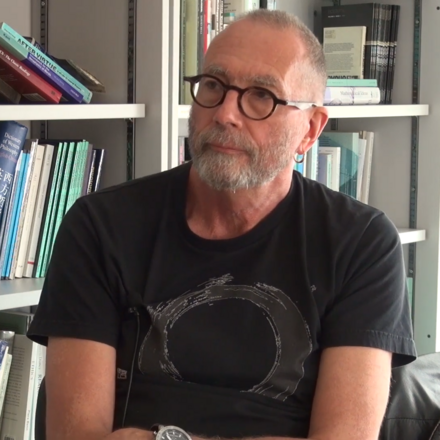
\includegraphics[width=0.6\textwidth]{priest.png}\\
    Graham Priest {\scriptsize\emph (Image by Wikipedia)}\\[3mm]
  \end{marginfigure}
Een voorbeeld van een dialetheia is \enquote{Deze zin is onwaar}. We kunnen deze zin als onwaar beschouwen, waardoor deze zou kloppen en dus tevens waar zou zijn. Als we deze zin als waar beschouwen, dan moeten we concluderen dat deze onwaar is. Een zin als deze wordt doorgaans als een paradox beschouwd en daarmee weggezet. Dialethe\"isme erkent het bestaan van dialetheia en probeert hier op een consistente manier meer te werken, waarbij verschillende paraconsistente logica's als formalisme gebruikt kunnen worden.
\end{aside}

\section{Modale Logica}\label{sec:modal}
Een modaliteit is een uitdrukking zoals \enquote{noodzakelijk} of \enquote{mogelijk}, die een waarheidswaarde kan be\"invloeden. In modale logica worden modaliteiten symbolisch binnen de logische taal weergegeven. Hiermee is modale logica, net als predicatenlogica, vooral een uitbreiding op een bestaand logisch systeem. Er bestaan verschillende modale logica's, elk met eigen interpetaties en axioma's. In de basis drukt modale logica noodzakelijkheid ($\Box A$, $A$ is noodzakelijk waar) en mogelijkheid ($\Diamond A$, $A$ is mogelijk waar), maar in deontische logica (die zich bezig houdt met ethische afwegingen) wordt dit bijvoorbeeld verplichting ($O$), toestaan ($P$) en verbod ($F$). Temporele logica (van \emph{tempus}, tijd) heeft het over ooit in het verleden ($P$), altijd in het verleden ($H$), ooit in de toekomst ($F$) en altijd in de toekomst ($G$). Doxastische logica gebruikt $BxA$ voor $x$ gelooft dat $A$, en Epistemische logica $KxA$ voor $x$ weet dat $A$; beide hebben toepassingen in game theory en bijvoorbeeld het raadsel van de \emph{muddy children}.

\begin{aside}[Muddy Children]
  Een groep kinderen\sidenote{... die allemaal kunnen redeneren en de basisprincipes van epistische logica kennen, zoals men zou verwachten ...} krijgt te horen dat tenminte een van hen modder op het gezicht heeft. Ieder kind kan het gezicht van alle anderen zien, maar niet van zichzelf, en mogen niet communiceren. Er wordt afgeteld, waarbij ieder kind dat weet dat het modder op het gezicht heeft gelijktijdig naar voren moet stappen. Als een kind foutief naar voren stapt wordt het gestrafd. Het proces herhaalt zich tot er alle kinderen met moddernaar voren zijn gestapt. Door zuiver redeneren kunnen de kinderen na een aantal iteraties zeker weten of ze wel of geen modder hebben; hoe?
\end{aside}

Wij zullen ons in deze sectie richten op de \enquote{basis}-variant van modale klassieke\sidenote{Het is mogelijk modaliteiten op verschillende logische systemen toe te passen; In de lineare logica is $\oc$ bijvoorbeeld ook een vorm van modaliteit. In de meeste gevallen waarin modale logica echte an sich bekeken wordt, is gebaseerd op een klassieke basis.} logica, die afhankelijk van gekozen aanvullende axioma's van verschillende interpretaties kan worden voorzien. We beperken ons daarmee tot de noodzakelijkheid $\Box$ en mogelijkheid $\Diamond$. Deze operatoren gedragen zich een beetje zoals respectievelijk $\forall$ en $\exists$, behalve dat ze geen variabele introduceren. Veel axioma's in de modale logica worden gedefinieerd aan de hand van $\Box$, waarbij $\Diamond$ kan worden gelezen als een notatie voor $\neg \Box \neg$ (iets dat noodzakelijk waar is, is onmogelijk onwaar).

De basis van het gros van de modale logica's is $\mathbf{K}$, dat naast de operatoren het axioma $\Box (A \to B) \to (\Box A \to \Box B)$ toevoegt (distributiviteit, ook wel axioma $K$). Daarnaast geldt voor elke $P$ dat $P$ een stelling in $\mathbf{K}$ is, dat $\Box P$ dit ook is.

Bovenop de modale logica $\mathbf{K}$ kunnen verdere axioma's toegevoegd worden. Een van de meest gebruikelijke is $\mathbf{T}$\sidenote{Soms ook bekend als $\mathbf{M}$.}, $\Box A \to A$. Als $A$ noodzakelijk waar is, dan is $A$ waar. Dit axioma wordt niet in elke vorm van modale logica's geaccepteerd --- in deontische logica zou dit vertalen naar $OA \to A$, en betekenen dat iedereen ook alles doet dat verplicht is; in temporale logica vertaalt dit naar $PA \to A$, alles dat altijd in het verleden het geval is geweest, is nu het geval (ook dit is, tot verdriet van veel Boomers, niet het geval).

Om semantiek te geven aan modale logica's wordt vaak gebruik gemaakt van een systeem van meerdere werkelijkheden, die met elkaar verbonden zijn. $\Box A$ betekent in dit geval dat $A$ waar is in alle werkelijkheden die met \enquote{onze} werkelijkheid\sidenote{De werkelijkheid van waaruit we redeneren.} onze werkelijkheid verbonden zijn, en $\Diamond A$ voor tenminste een van die werkelijkheden. Als twee werkelijkheden $w_0$ en $w_1$ met elkaar verbonden zijn, zodat modaliteiten in $w_0$ invloed hebben op $w_1$, dan schrijven we $w_0 > w_1$. Merk op dat nog nergens gesteld is dat onze werkelijkheid met zichzelf verbonden is, of dat die verbinding twee kanten op gaat. Binnen $\mathbf{K}$ geeft $\Box A$ aan dat in alle werkelijkheden die op de onze volgen, $A$ waar is, maar niet per definitie in onze eigen werkelijkheid. Dankzij het axioma $\mathbf{T}$ is dit in de gelijknamige logica $\mathbf{T}$ wel het geval en geldt $w_n > w_n$.

Een volgend axioma dat kan worden toegevoegd is $\mathbf{B}$: $A \to \Box \Diamond A$. Tezamen met $\mathbf{T}$ levert dit de logica $\mathbf{B}$ op. Het axioma stelt dat als $A$ waar is, dat dit in alle werkelijkheden die we kunnen bereiken mogelijk is, dus dat voor elk van deze werkelijkheden geldt dat we een werkelijkheid kunnen bereiken waar $A$ waar is. Deze werkelijkheid, die in alle richtingen 2 stappen van ons verwijderd is, is onze eigen werkelijkheid, wat betekent dat als we van werkelijkheid $w_0$ naar $w_1$ kunnen komen, we van $w_1$ weer terug in $w_0$ kunnen komen, oftewel $w_n > w_m \iff w_m > w_n$.

Alternatief kunnen we de axioma's $\mathbf{4}$ of $\mathbf{5}$ toevoegen aan $\mathbf{T}$ om met series modaliteiten om te gaan. $\mathbf{4}$ stelt $\Box A \to \Box \Box A$, en heeft tot gevolg dat we een serie gelijke modaliteiten tot \'e\'en kunnen samenvoegen\sidenote{Overtuig jezelf dat $\mathbf{4}$, die met $\Box$ gegeven is, voldoende is om deze uitspraak ook over $\Diamond$ te doen; gebruik hierbij de definitie van $\Diamond$ die eerder gegeven is.}. Concreet komt dit erop neer dat als $w_0 > w_1$ en $w_1 > w_2$, ook geldt dat $w_0 > w_2$. We mogen met dit axioma dus werkelijkheden overslaan. De logica met $\mathbf{K}$, $\mathbf{T}$ en $\mathbf{4}$ wordt $\mathbf{S4}$ genoemd. In plaats daarvan kunnen we ook axioma $\mathbf{5}$, $\Diamond A \to \Box \Diamond A$ , nemen om $\mathbf{S5}$ te krijgen. Hier kunnen we elke serie modaliteiten tot \'e\'en samenvoegen, en hoeven we allen de laatste te behouden. Als we $\mathbf{B}$ aan $\mathbf{S4}$ toevoegen krijgen we overigens precies dezelfde logica $\mathbf{S5}$.

De hier genoemde axioma's en systemen zijn de meest gangbare, maar zeker niet de enige modale systemen. De sequenten-regels overeenkomend met de axioma's staan gegeven in Stelling~\ref{th:sq-modal}.

\begin{figure}[ht]
\begin{theorem}\label{th:sq-modal} Regels voor modale logica
\mbox{}\\[3mm]
\inference{\Box_K}{\Gamma \vdash A}{\Box \Gamma \vdash \Box A}
\hspace{5mm}
\inference{\Box_T}{A, \Gamma \vdash \Delta}{\Box A, \Gamma \vdash \Delta} \\

\vspace{4mm}

\inference{\Box_4}{\Box \Gamma \vdash A}{\Box \Gamma \vdash \Box A}
\hspace{5mm}
\inference{\Box_5}{\Box \Gamma \vdash \Box \Delta, A}{\Box \Gamma \vdash \Box \Delta, \Box A}
\end{theorem}
\end{figure}
